\section{Project Plan}

The project plan provides a rough outline of all sprints, main activities and their respective time-frames represented as a Gantt-chart. The project is divided into nine sprints of about two weeks, and each sprint has it´s unique goal. The last sprints are not planned in full detail to give us a time buffer for unseen time and feature creep.

\subsection{Presentations}
During the project we will have three presentations. One presentation in the start phase of the project, one presentation in the middle of the project and one presentation at the end of the project. A short description of what the different presentations shall include is below. \\\\
\begin{figure}[h]
\begin{minipage}[t]{0.5\textwidth}
\textbf{Presentation 1:}
\begin{itemize}
  \item Who we are
  \item What we will do
  \item How we will do it
  \item Describe the process 
  \item What will happen next? 
  \item Project plan
  \item Requirement specification
  \item Test specification 
\end{itemize}
\end{minipage}
\hfill
\begin{minipage}[t]{0.5\textwidth}
\textbf{Presentation 2:}
\begin{itemize}
  \item Our chosen design
  \item How testing is performed
  \item What has been done
  \item Progress 
  \item What's next
\end{itemize}
\end{minipage}
\hfill
\end{figure}\\
\\
\textbf{Presentation 3:}
This presentation is divided into two main parts of 20 minutes. The first part is sales pitch of the product. The second part is a technical presentation of the product. \\
The first part shall describe:
\begin{itemize}
  \item Why our product/solution is the best 
  \item Mention the positive sides of the product
  \item Compare our product to other products 
\end{itemize}
The second part shall describe: 
\begin{itemize}
  \item What we have learned during the project 
  \item Our time-consumption 
  \item The technical solution
  \item A conclusion of the project 
\end{itemize} 

\subsection{Milestones}
In order to complete this project, we have made a list of our intended milestones. The milestones represent the important events within a projects life time and when it is expected to be accomplished. Milestones can be considered as a short summary of when these activities should be finished. Milestones are composed of tasks that are too large to have a meaningful duration assigned to it. 
\\\\
Some of the intention behind milestones is to gain insight and understanding of the tasks to be solved. The milestones give an overview of the work to be done, and a base for committing resources. The goal is to have a good overview of the progress in the project. The Gantt-chart however, gives a detailed overview of all activities in the entire project from start to finish. Milestones are a way to summarize tasks into larger pieces and keep track of the project development. They give a clear deadline for when these tasks should be done. Deadlines are set to have a greater efficiency and progress. It provides information to the stakeholders of what they can expect of progress and when the various stages will be completed.\\
\begin{table}[h]

\centering\section*{\textbf{Milestones}}
\caption{Milestones}
\begin{tabular}{llc}
\rowcolor{cadetgrey}
\centering \textbf{Milestone:}    &\textbf{Description:} 	 &\textbf{Expected done:} \\ % &\textbf{Main responsibility:}  \\

\rowcolor{gainsboro}
\textbf{Requirements Identification} & Identify requirements and needs & $13.01.17$ \\
\textbf{Project Plan} & Create a project plan, divide activities, & $24.01.17$ \\
                                     & plan organization & \\
\rowcolor{gainsboro}
\textbf{First Prototype} & Create a simple fixed pitch & $14.02.17$ \\\rowcolor{gainsboro}
                         & quadcopter to test & \\\rowcolor{gainsboro}
                         & flight controller & \\
\textbf{Preliminary Design} & Create a preliminary design & $21.02.17$ \\
                            & for fixed and variable pitch & \\\rowcolor{gainsboro}
\textbf{Basic PID controller} & Develop basic PID controller & $21.02.17$ \\\rowcolor{gainsboro}
                                 & For a fixed and & \\\rowcolor{gainsboro}
                                 & variable pitch quadcopter & \\
\textbf{Basic Flight Controller} & Create a basic flight controller & $28.02.17$ \\
                                 & so the quadcopter can elevate, & \\
                                 & land and go left and right & \\\rowcolor{gainsboro}
\textbf{Fixed Pitch Quadcopter} & Create the fixed pitch quadcopter & $13.03.17$ \\\rowcolor{gainsboro}
                                & (no more changes have been planned) & \\
\textbf{Flight Controller FPQ}  & Finish a flight controller for fixed & $28.03.17$ \\
                                & pitch with possibility for autonomous & \\
                                & and agile flying & \\\rowcolor{gainsboro}
\textbf{Variable Pitch Quadcopter}  & Create the variable pitch quadcopter & $14.03.17$ \\\rowcolor{gainsboro}
                                    & (no more changes have been planned) & \\
\textbf{Flight Controller VPQ}  & Finish a flight controller for variable & $28.03.17$ \\
                            & pitch with possibility for autonomous & \\
                            & and agile flying & \\\rowcolor{gainsboro}
\textbf{Compare fixed and variable pitch}  & Test and compare the quad- & $14.04.17$ \\\rowcolor{gainsboro}
                                           & copters to answer the main & \\\rowcolor{gainsboro}
                                           & requirements & 
\end{tabular}                                                               
\end{table}

\subsection{Activity List}

The purpose of identifying the project activities is to get a sufficient estimate on what resources and time the project will require to be completed. Activities are usually given an expected duration and resource use, in terms of manpower, knowledge and budget. 
The list tends to be extensive containing all scheduled activities in the project. Scrum on the other hand doesn't plan when every activity should be done. The first phase in a scrum project is to make a product roadmap, which can be done in as little as a day. Scrum gets an advantage by cutting the planning process, but in return struggles with getting the project done within a given time-frame. Since we can't move the end date of the project, Scrum needs to be modified a little in order to meet our project needs. \\
\\
We will in our project do a mix of the traditional long-term planning and Scrum. Planning for all the project sprints as well as using the advantage of scrum by planning each sprint in-depth. Combining the sprints with an overall project plan helps by reaching the end date and still keep Scrum's feedback and agility.
 You can find a list of the initial activities that we have identified at this point in the project beneath. \\
\\
The process of identifying activities uses decomposition to break down the structure of larger tasks (such as milestones and backlog items). Activities identified by asking "What has to be done" often in form of functionality. We then take the functionality and translate it into milestones and larger activities. 
\begin{center}
\centering\section*{\textbf{Activity Layout}}
%\caption{Activity Layout 1}
\begin{tabular}{cllll}
\rowcolor{cadetgrey}
\textbf{ID:}    &\textbf{Activity:} 	 &\textbf{Estimated time:}    &\textbf{Start:}  \\ % &\textbf{Main responsibility:}  \\
    
\textbf{1} & \textbf{Start-Up Phase} & \textbf{260h} & $03.01.17$ 
\\\rowcolor{gainsboro}
1.1       & Documentations     &     &  \\
1.2       & Research     &     &  \\\rowcolor{gainsboro}
1.3       & Project Model     &     & \\
1.4       & Project Plan     &     & 
\\\rowcolor{gainsboro}
1.5       & Requirements     &     & \\
1.6       & Test Specification     &     & 
\\\rowcolor{gainsboro}
1.7       & Document Templates     &    & \\
1.8       & Internal Meetings      &    & 
\\\rowcolor{gainsboro}
1.9       & External Meetings      &    & \\
\textbf{2} & \textbf{Presentation 1}     & \textbf{100h}    & $03.01.17$ 
\\\rowcolor{gainsboro}
2.1     & Preliminary Documentation Refinement  &    & \\
2.2     & Presentation Refinement  &    &
\\\rowcolor{gainsboro}
2.3     & Presentation Practice  &    & \\
\textbf{3} & \textbf{Sprint 1}     & \textbf{360h}     & $17.01.17$ 
\\\rowcolor{gainsboro}
3.1     & First Presentation &  & \\
3.2     & Preliminary Flight Simulation &  & 
\\\rowcolor{gainsboro}
3.3     & Communication With Qualisys &  & \\
3.4     & Mechanical Design Study &  & 
\\\rowcolor{gainsboro}
3.5       & Internal Meetings      &    & \\
3.6       & External Meetings      &    & 
\\\rowcolor{gainsboro}
\textbf{4} & \textbf{Sprint 2}     & \textbf{360h}     & $31.01.17$ \\
4.1     & Electrical Analysis &  &  \\\rowcolor{gainsboro}
4.2     & Electrical Layout &  & \\
4.3     & Electrical Construction & & \\ \rowcolor{gainsboro}
4.4     & Flight Controller & & \\
4.5     & Create Web Page & &  
\\\rowcolor{gainsboro}
4.6     & Mechanical Design & & \\
4.7     & Preliminary Construction & & 
\\\rowcolor{gainsboro}
4.8       & Internal Meetings      &    & \\
4.9       & External Meetings      &    & 
\end{tabular}                                                                   
\end{center}
\newpage

\begin{center}
\section*{\textbf{Activity Layout}}
%caption{Activity Layout 2}
\begin{tabular}{cllll}
\rowcolor{cadetgrey}
\textbf{ID:}    &\textbf{Activity:} 	 &\textbf{Estimated time:}    &\textbf{Start:}  \\ % &\textbf{Main responsibility:}  \\
\rowcolor{gainsboro}
\textbf{5} & \textbf{Sprint 3}     & \textbf{360h}     & $14.02.17$ \\
5.1     & Plan Test Procedures &  &  \\\rowcolor{gainsboro}
5.2     & Mechanical Design &  &  \\
5.3     & Preliminary Variable Pitch Design & & 
\\\rowcolor{gainsboro}
5.4     & Flight Testing and Controll &  & \\
5.5       & Internal Meetings      &    & 
\\\rowcolor{gainsboro}
5.6       & External Meetings      &    & \\
\textbf{6} & \textbf{Sprint 4}     & \textbf{360h}     & $28.02.17$ \\
\rowcolor{gainsboro}
6.1     & Mechanical Design Review & & \\
6.2     & Tweak Flight Controller & & 
\\\rowcolor{gainsboro}
6.3       & Internal Meetings      &    & \\
6.4       & External Meetings      &    & 
\\\rowcolor{gainsboro}
\textbf{7} & \textbf{Sprint 5}     & \textbf{360h}     & $14.03.17$ \\
7.1     & Advanced Controll Functionality &  & \\\rowcolor{gainsboro}
7.2       & Internal Meetings      &    & \\
7.3       & External Meetings      &    & 
\\\rowcolor{gainsboro}
\textbf{8} & \textbf{Presentation 2}     & \textbf{100h}     & $28.03.17$ \\
8.1     & Presentation 2 planning &  &  \\\rowcolor{gainsboro}
\textbf{9} & \textbf{Sprint 6}     & \textbf{360h}     & $28.03.17$ \\
9.1     & Finalize Test Procedures &  & 
\\\rowcolor{gainsboro}
9.2     & Tweak Controller System &  & \\
9.3       & Internal Meetings      &    & 
\\\rowcolor{gainsboro}
9.4       & External Meetings      &    & \\
\textbf{10} & \textbf{Sprint 7}     & \textbf{460h}     & $11.04.17$ \\
\rowcolor{gainsboro}
10.1     & Final Flight Controller Adjustment &  & \\
10.2     & Testing and Comparison & & 
\\\rowcolor{gainsboro}
10.3       & Internal Meetings      &    & \\
10.4       & External Meetings      &    & 
\\\rowcolor{gainsboro}
\rowcolor{gainsboro}
\textbf{11} & \textbf{Sprint 8}     & \textbf{460h}    & $25.04.17$ \\
11.1     & Testing and Comparison              &  &  \\\rowcolor{gainsboro}
11.2     & Documentation &  &  \\
11.3     & Testing & &  \\\rowcolor{gainsboro}
11.4       & Internal Meetings      &    & \\
11.5       & External Meetings      &    & 
\\\rowcolor{gainsboro}
\rowcolor{gainsboro}
\textbf{12} & \textbf{Sprint 9}     & \textbf{460h}     & $09.05.17$ \\
12.1     & Testing and Comparison &  &  \\\rowcolor{gainsboro}
12.2     & Documentation Review &  & \\
12.3       & Internal Meetings      &    & 
\\\rowcolor{gainsboro}
12.4       & External Meetings      &    & \\
\textbf{13} & \textbf{Presentation 3}     & \textbf{100h}     & $09.05.17$ \\
\rowcolor{gainsboro}
13.1     & Documentation Review &  & \\
13.2     & Practice & & \\
\rowcolor{gainsboro}
         & \textbf{Total amount of hours estimated:} & \textbf{4200h} & 
         \\\\\\\\\
\end{tabular}                                                               
\end{center}


\subsection{Gantt-chart}

Imagine being a juggler, juggling a lot of balls. The more balls you have in the air, the harder it gets keeping track of everything. In addition the more balls we have in the air, the more mess it can potentially be if something starts to slip out of hand. Being a juggler and being a system engineer are similar when it comes to this. The engineer needs to keep track of all the activities in the project, if he does not accomplish this, then the project will surely fail. Failure to deliver a task or a sequence of tasks within a given deadline, can have direct or indirect effect on the rest of the project. This may affect the end date of the project as well as the cost.\\
\\
This is why it is advantageous to have an overview of the project and its associated tasks. With a Gantt chart you could see all this information at a glance. Usually, the most critical activities and milestones are represented in the Gantt-chart. Gantt-charts are an important tool when it comes to visualisation of activities. It's frequently used in project management, and are closely followed up by the project leader in order to meet the deadline. The chart has a list of the tasks on the left and information about the start, duration, relationship to other tasks and end date as a timeline to the right. The Gantt-Chart is provide as a seperate document. \\

\begin{comment}
Things that should be in a project plan/ description:

Scope management
Schedule management
Financial management
Quality management
Resource management
Stakeholder management – New from PMBOK 5[citation needed]
Communications management
Project change management
Risk management
\end{comment}

\subsection{Budget}
The project has a budget of 10.000 NOK. The budget will mainly be used to purchase quadcopter parts. A small amount of the budget is used on project management tools, such as Jira and sharelatex. If we encounter unforeseen expenses, FFI has approved that the budget may be stretched to 15.000 NOK.
\\\\

\csvautotabular{budget.csv}
Here is our budget so far.

\subsection{Risk Management}
During the start-up phase of a project it is important to do a thorough risk analysis, so that we can be reactive to scenarios that could endanger our project. A risk is something that can put the project at danger in any way. The risk analysis identifies all possible scenarios that can cause problems for the project development, and determines the probability and severity of these. By identifying these scenarios we can minimize, or eliminate the risks. It is important to always reevaluate the risks at every sprint, in order keep track of current risks or identify new ones.
\newline \newline
Examples of risk scenarios are budget overrun, injuries, long term sick-leave etc. The scenarios is categorized with the probability of occurrence and the severity of this scenario. The scenarios are further analysed in a risk matrix which helps us to see which risks are most critical for the project.\newline \newline
We used three categories to analyze the risk scenarios.
\begin{itemize}
\item{Likelihood of occurrence.}
\item{Severity of the scenario.}
\item{ Detectability(How easy it is to detect the risk scenario.)}
\end{itemize}
All risk scenarios are rated according to these three categories with low, medium and high ranking. A likelihood of high, means that the scenario is most likely to happen. High severity means that the consequences are severe if it happens. And high detectability means that it is hard to detect the scenario.\newline \newline
Three strategies of action(SOA) were used to treat the risks.
\begin{itemize}
\item{Accept: The risks with a low ranking got accepted. No action is needed on these. No imminent danger}
\item{Protect: Risks with medium ranking requires some actions to reduce the probability of occurrence.}
\item{Avoid: Risks with high ranking. These risks need to be eliminated or reduced. If the risk occurs, a plan to handle the risk needs to be developed.}
\end{itemize}
Figure \ref{fig:risk} shows all the different risk scenarios, along with the strategies, likelihood, severity and detectability, origin. Every scenario has an unique ID for traceability.
\begin{figure}[H]
    \centering
    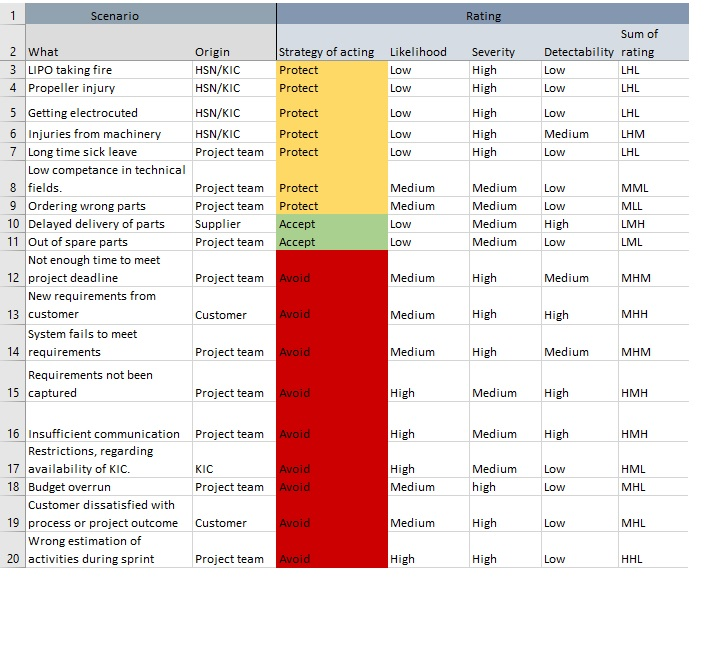
\includegraphics[width = 1.0\textwidth]{VAPIQ-PICTURES/RiskScenarios.jpg}
    \caption{Risk scenarios with ratings}
    \label{fig:risk}
\end{figure}
\noindent We developed a risk assessment matrix, as seen in figure \ref{AssRisk}. This table is a very helpful tool to visualize the risk, and how critical it is.
\begin{figure}[H]
    \centering
    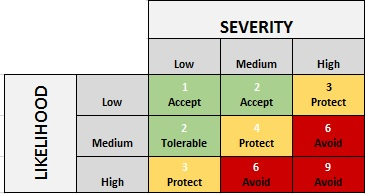
\includegraphics[width = 0.3\textwidth]{VAPIQ-PICTURES/Riskmatrix.jpg}
    \caption{Risk assesment matrix}
    \label{AssRisk}
\end{figure} \\
\noindent
A risk is defined as the product between the probability of occurrence times the severity. Risk = likelihood$\cdot$severity. Which SOA(stategy of action) we are going to use is determined from the risk assessment table.
\newline \newline
After analysing all scenarios in the risk assessment matrix, we know that sudden new requirements from the customer FFI, can put the project at risk. This is because of limited time and a deadline that is fixed. If this happens we need to adapt and accept it, change the backlog and re-prioritize activities. And since we are using the highly iterative scrum model, it is relatively easy to handle changes.The risk which got the highest rating was wrong estimation of story-points. Estimating wrong will put the whole project in danger in the way that we don't have a product at the end. Most of the highest risks, are connected to requirements. Thus we need to always reevaluate user stories at every sprint review meeting in order to ensure completeness. Budget overrun also is a huge risk. Therefore it is important to do thorough studies before we decide to order parts.\newline \newline
To ensure low risk it is important to have a risk meeting at the beginning of each sprint. Here we reevaluate the risk scenarios, and analyzes which risks that are most likely to happen during the sprint. During these meetings we must develop plans on how to handle the risks that are most likely to happen.